%!TEX root = paper.tex
%%%%%%%%%%%%%%%%%%%%%%%%%%%%%%%%%%%%%%%%%%%%%%%%%%%%%%%%%%%%%%%%%%%%%%%%%%%%%%%
\section{User Perspective and Prospects}
\label{sec:engagement}

In this section we interpret the previous results from the point of view of an end customer. Section~\ref{subsec:metrics} reviews game and platform characteristics as possible engagement metrics, i.e. measures for the attractiveness of a platform. Section~\ref{subsec:cost-benefit-models} constructs two simple cost/benefit models based on the platform costs and the number of games affordable as a benefit metric.


%%%%%%%%%%%%%%%%%%%%%%%%%%%%%%%%%%%%%%%%%%%%%%%%%%%%%%%%%%%%%%%%%%%%%%%%%%%%%%%%
\subsection{Engagement Metrics}\label{subsec:metrics}

The benefit that platform and game characteristics create for different types of gamers are diverse. We try to reflect this diversity in our interpretations.

%Metrics for user engagement, defined as ``\textit{the quality of the user experience that emphasises the positive aspects of the interaction, and in particular the phenomena associated with being captivated by a web application, and so being motivated to use it}''\cite{Lehmann2012}, can be used to compare different services against each other. The problem with engagement is finding the right measures befitting the type of service under scrutiny, in this case gaming, and cloud gaming in particular.
%So, which platform characteristics engage gamers? Compared to video content and video streaming platforms this is harder to answer due to the high diversity of both games and  gamers. Looking at some simple summary metrics in Tab.~\ref{tab:game-stats} does not give a clear picture, with one exception: the number of titles. 

%Due to the nature of the Cloud services (streaming existing games) there are no ``platform exclusive'' titles, which often increases the attractiveness of a specific platform for specific audiences. These limits on variety might be one reason why \steam is much more compelling to wider audiences.
%\footnote{PZ: Theoretically a game could be exclusive on a specific cloud service platform, which may not be good choice due to the small market, but theoretically it could work. Or not?}
%AR: If https://en.wikipedia.org/wiki/List_of_PC_exclusive_games is to be trusted, (now-defunct cloud gaming service) OnLive did have exclusive titles: "Armada 2526'" and "Vanguard Princess".

\subsubsection{Number of games} The number of games for the three platforms are widely dissimilar, making the choice unanimous for gamers that favour wider ranges of offers. Other factors motivating different platform choices might be found in already-owned console hardware, or hypothetical platform-exclusive titles.

\subsubsection{Age of games} This has multiple possible effects on attractiveness. Older games might be more likely to be considered ``classics''. On the other hand, newer games tend to also be topics in the media (and in advertising, increasing their publicity), offer a greater diversity (e.g. regarding game mechanics and control), % Wii once was new!
and feature improved technical quality (resolution, scene complexity).

\subsubsection{Game lenghts} We argue that engagement due to game length should be considered differently depending on the player type. For casual gamers, shorter games probably have more appeal, as their limited playtime is more likely to allow players to complete them. ``Hard core'' gamers that spend more time gaming overall might find longer games more engaging. If a gaming platform wants to attract members of both crowds, it should thus offer a wide range of game lengths. 
Figure~\ref{fig:rel-combinedlength-owners} plots the number of owners of games on  \steam over the combined game length from the \hltb dataset. A small positive effect exists (Pearson correlation $= 0.175$), indicating that longer games attract more buyers, or (swapping cause and effect) that more people tend to buy longer games.
% The playthrough time may be an indicator for the amount of provided content (albeit not the quality).

\subsubsection{Review scores} Published scores for games constitute an additional social factor, in that gamers might be drawn to positively-reviewed titles more strongly. Taking game ownership as a possible indicator for the popularity of a game, we find from the \metacritic dataset a small positive correlation between general score and number of game ownerships on \steam (Pearson correlation coefficient $= 0.199$).
%Interestingly, for \metacritic user scores the effect turns out to be smaller (Pearson correlation $= 0.101$). The influence of experts' scores turns out to have a greater influence (though still somewhat small) on the buying decision than the users' scores.


\begin{figure}[!t]
	\centering
	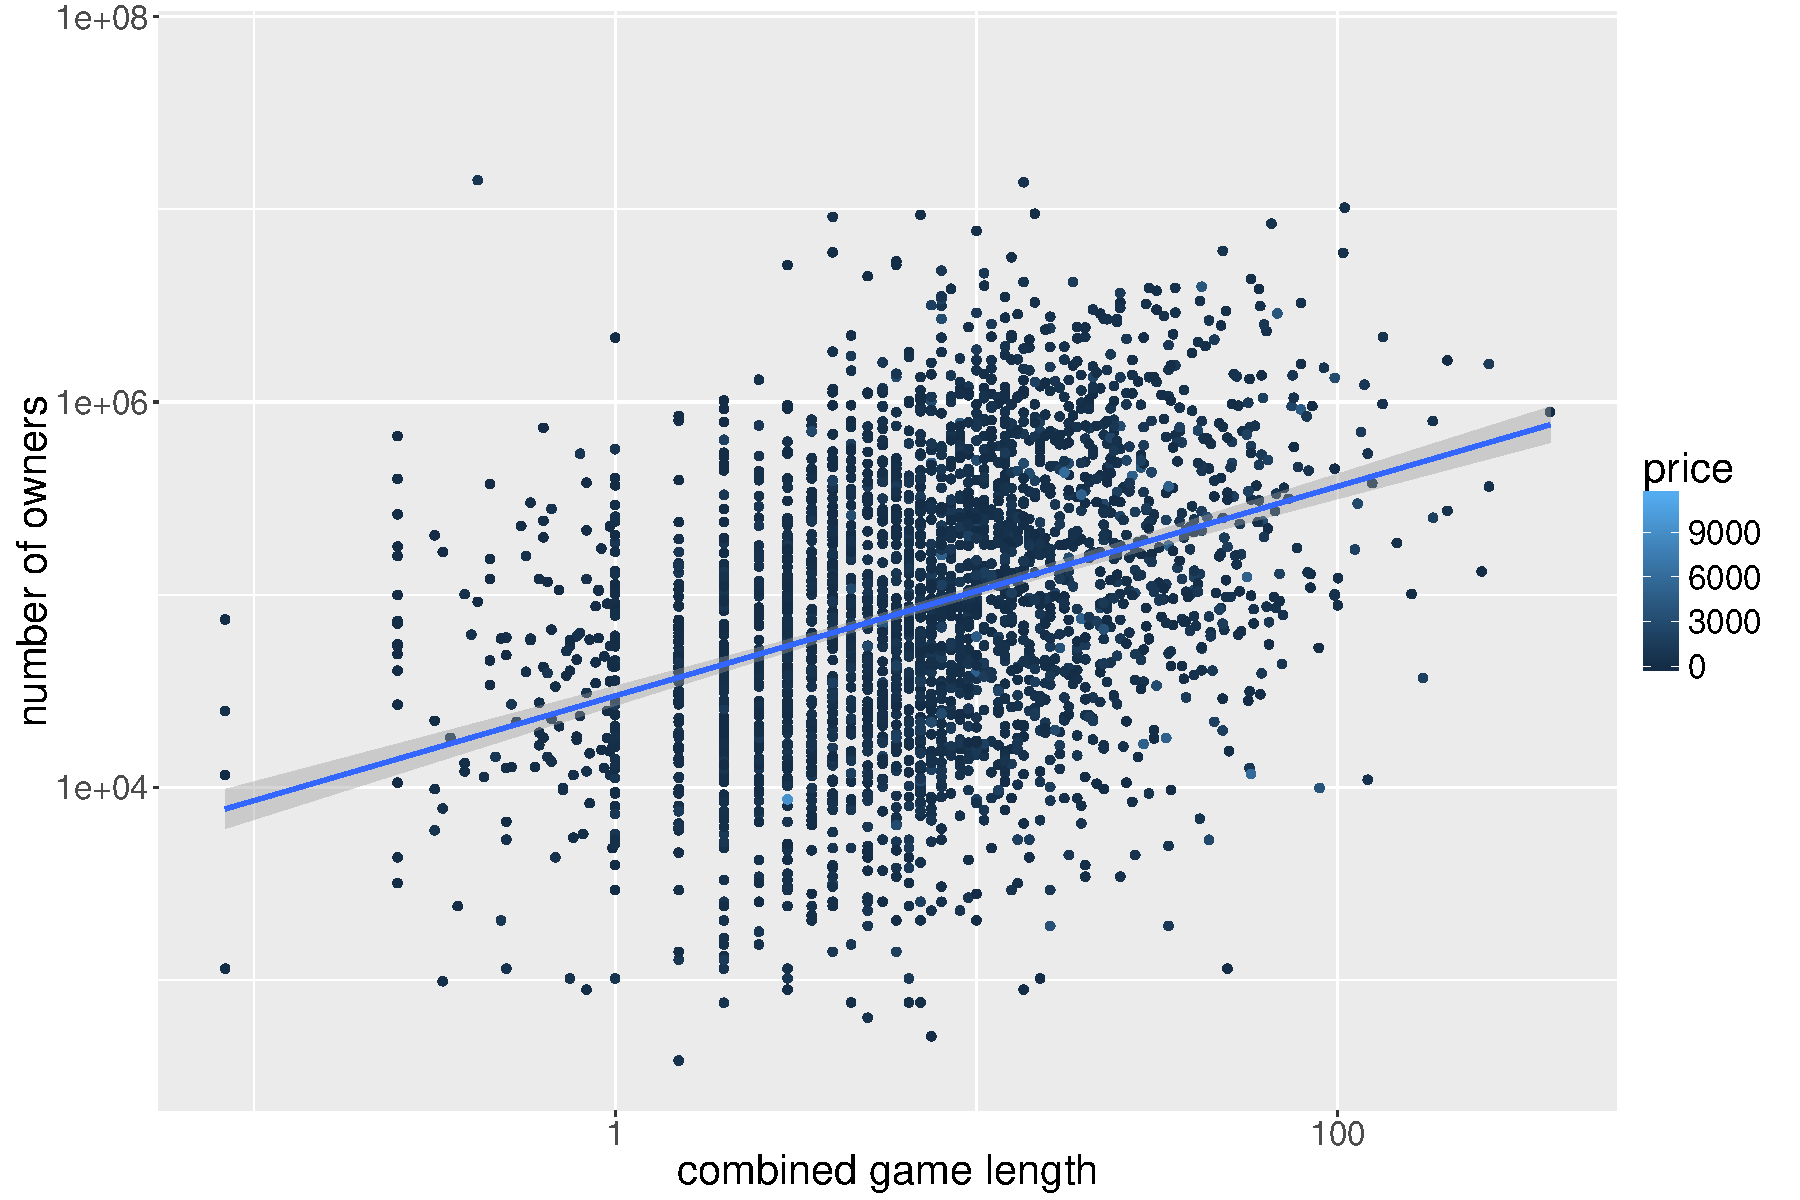
\includegraphics[width=1.0\columnwidth]{images/rel-combinedlength-owners.pdf}
	\caption{Relationship game length to ownership}
\label{fig:rel-combinedlength-owners}
\end{figure}


%%%%%%%%%%%%
\subsubsection{Further Potential Engagement Factors}

Due to the limited amount of available data the number of currently observable potential engagement metrics is restricted. However, many more come to mind and are worth investigating in the future. These could include,

\begin{itemize}
	\item the number of platform ``exclusive'' game titles,
	\item the genre as well as other classifications of games,
	\item the number of game sales and subscriber numbers,
	\item technical aspects like graphical fidelity, performance, precision and responsiveness of controls,
	\item measures of the game's content like variety and quality of game mechanics,
	\item or other content-centric factors.
\end{itemize}




%However, when having a look at figures \ref{fig:rel-price-category-owners} and \ref{fig:rel-score-category-owners}, 
%Some details remain unclear: Despite having a relatively low Metacritic score, especially games within the 11-20 range seem to have quite a number of owners - why? Also, either games for free or expensive games seem to be popular. Maybe this is an indicator for the differentiation between hardcore and casual gamers? (Probably it would be interesting as well to track the price over the years and also weigh the ownership count relatively to a game's age.)

%\begin{figure}[!t]
%	\centering
%	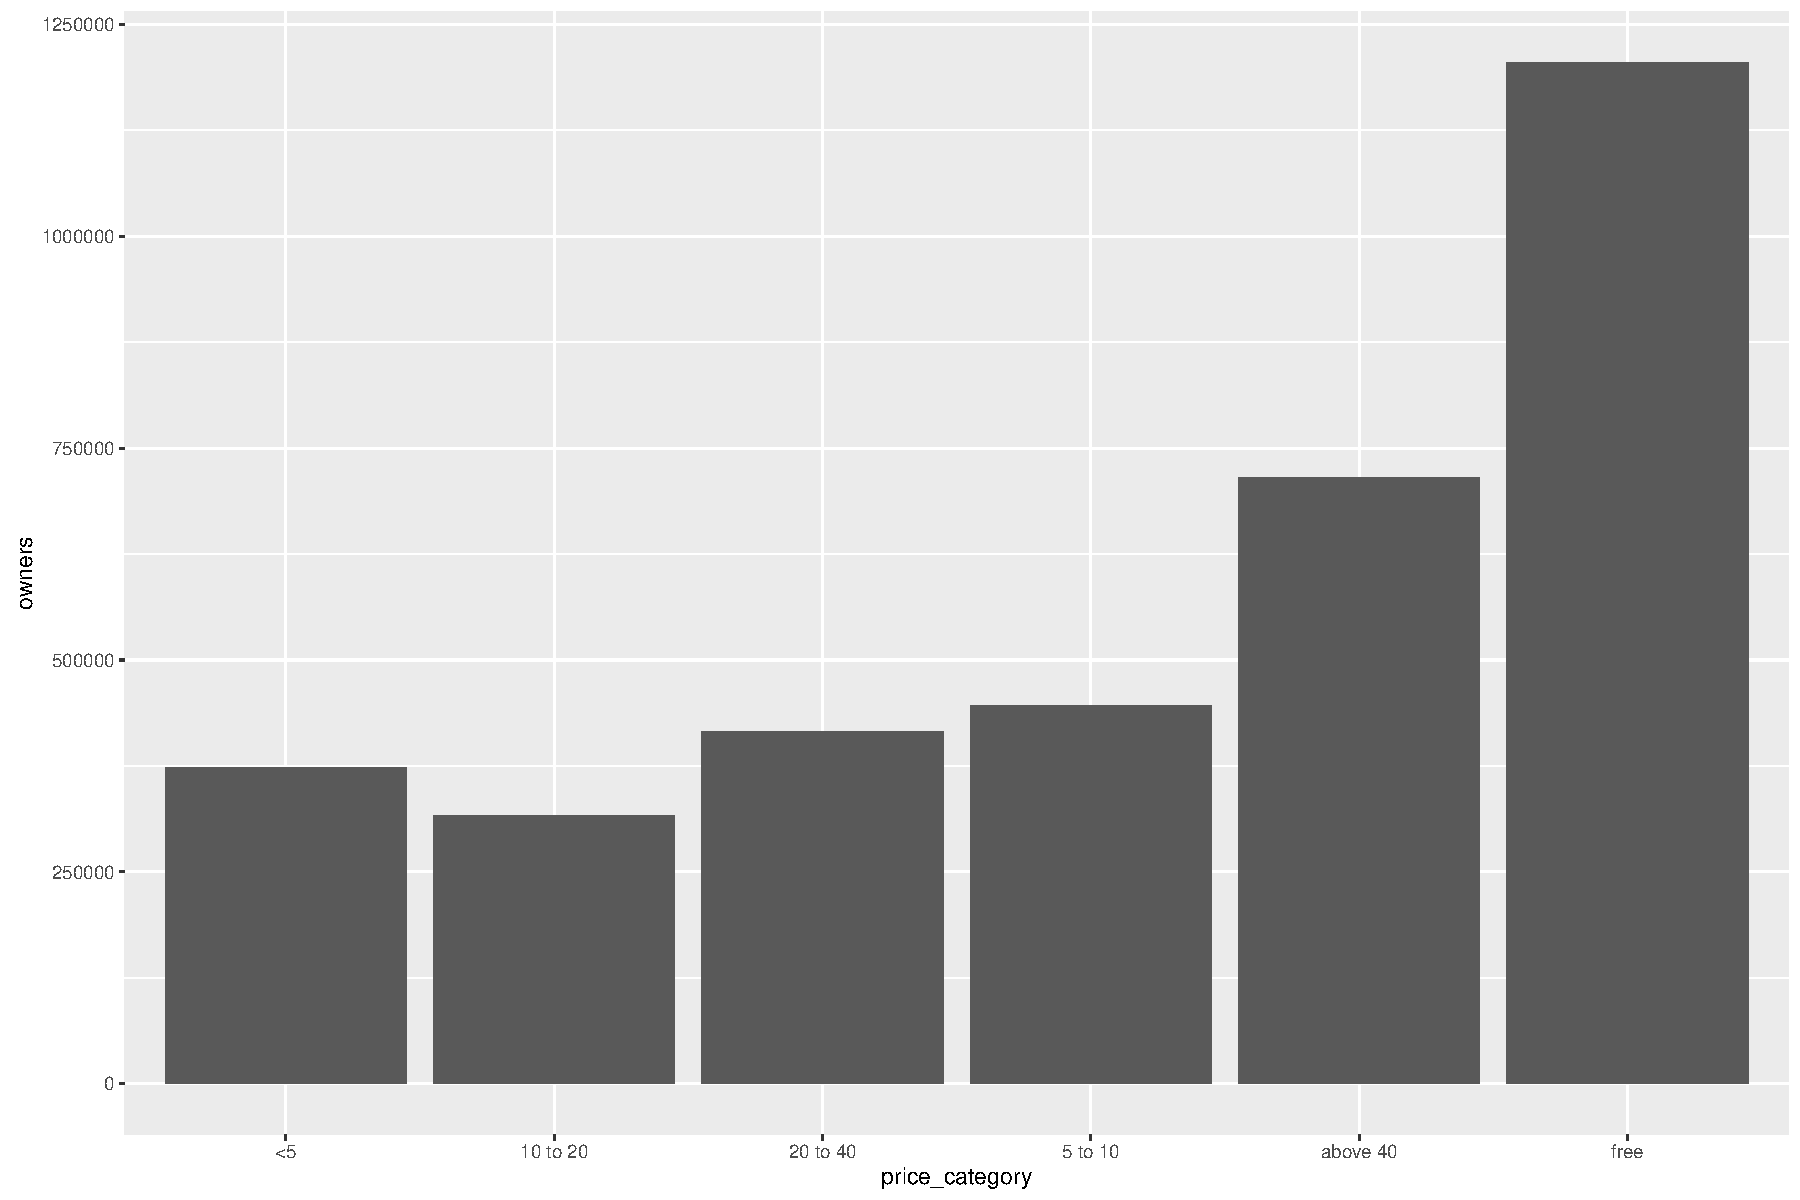
\includegraphics[width=1.0\columnwidth]{images/rel-price-category-owners.pdf}
%	\caption{Relationship price category to ownership (\textbf{TODO: Bars need sorting})}
%\label{fig:rel-price-category-owners}
%\end{figure}
%
%\begin{figure}[!t]
%	\centering
%	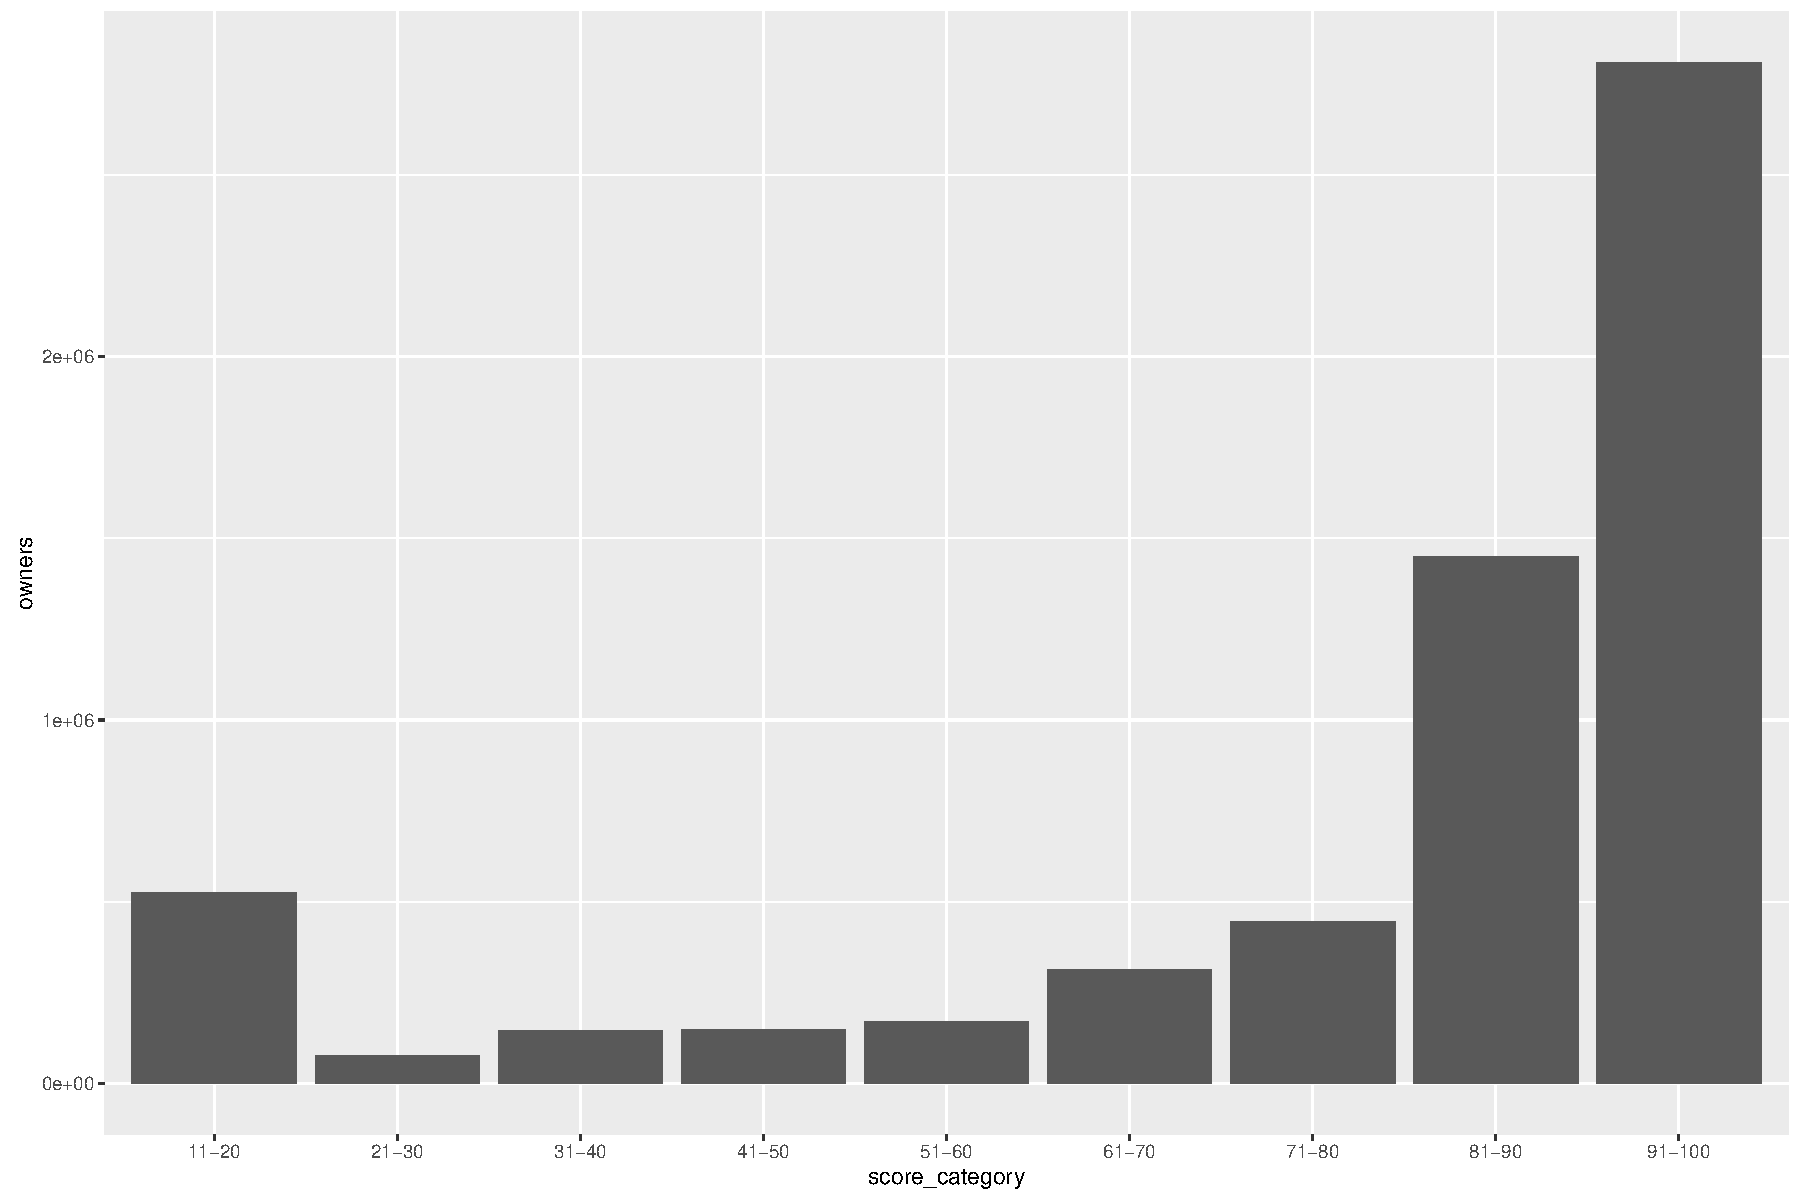
\includegraphics[width=1.0\columnwidth]{images/rel-score-category-owners.pdf}
%	\caption{Relationship score category to ownership (\textbf{TODO: Bars need sorting})}
%\label{fig:rel-score-category-owners}
%\end{figure}




%%%%%%%%%%%%%%%%%%%%%%%%%%%%%%%%%%%%%%%%%%%%%%%%%%%%%%%%%%%%%%%%%%%%%%%%%%%%%%%%
\subsection{Cost-Benefit Models}


The price models for cloud services, as deliberately excluded in the discussion of engagement metrics, largely differ from the approach of \steam. Setting the number of games, as noteworthy value metric, in relationship to the cost or budget (service price), two simple models are created. Naturally, this does not factor in any user preferences to specific games and their availability on just a subset of platforms. But the current curated nature of Cloud Gaming platforms would prevent this endeavour from succeeding regardless.

\todo[inline]{PZ: Which models? Or what are the models?}

%Moreover, the examined engagement metrics do not provide many means for a service distinction bar the number of games available. Therefore, the two simple models provided here use the number of affordable games on a specific budget. 

For both models a few basic assumptions are made. The initial hardware costs are factored in proportionately to the expected life and depreciation time of the devices, which is assumed to be \SI{3}{\year} for PCs and \SI{7}{\year} for the consoles and devices necessary to receive the streaming service (\SI{7}{\year} is about the average life cycle of a video game console generation and should be representative in this case).

What should also be noted is the difference in the service model between the ownership model of \steam, the hybrid subscription plus permanent rental model of \gfnow, as well as the subscription and timed rental model of \psnow. For the latter rentals subscription is also not a prerequisite. As this subtle differences are difficult to express in a simple cost-benefit model, they are all treated the same here. Therefore, they are all treated equally in the models as games, that one has access to and could have been played at one point. Other means of acquiring games cheaper from outside of the respective services, of which there are many for PC gaming as discussed in Sec.~\ref{sec:pcgaming}, are also omitted here.

%%%%%%%%%%%%%%%%%%%%%%%%%%%%%%%%%%%%%%%%%%%%%%
\paragraph{Affordable Games on a Budget Model}

The first model assumes that one has a fixed budget to spend on video games. This model then shows, depending on the size of the budget, how many games one would be able to afford considering all initial and continual costs.

\begin{figure}[!t]
	\centering
	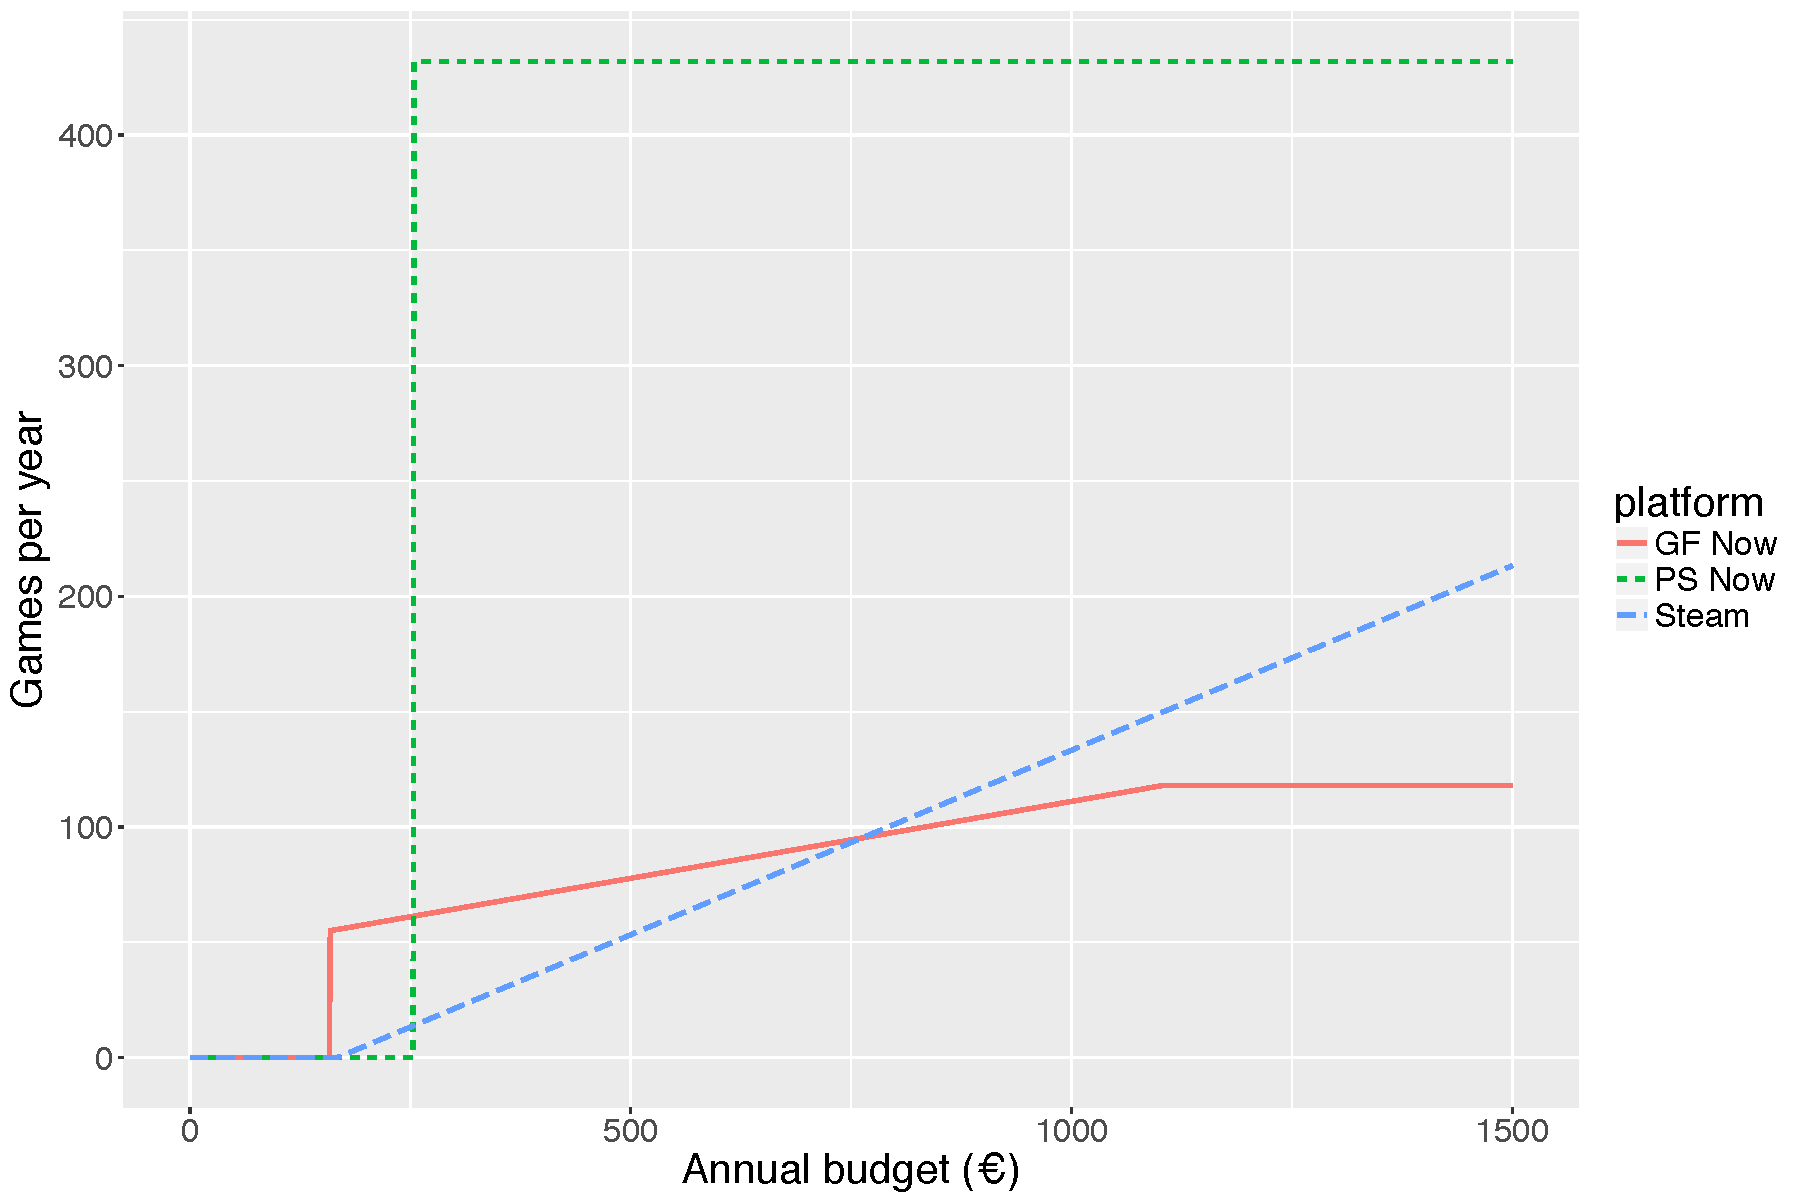
\includegraphics[width=1.0\columnwidth]{images/gamesperyear-over-budget.pdf}
	\caption{Per-platform price models as relationship of offered games (y-axis) in customer expenditure (budget; x-axis).}
\label{fig:gamesperyear-over-budget}
\end{figure}

As evident in Fig.~\ref{fig:gamesperyear-over-budget} all platforms start with relatively high fix costs, but only the subscription models provide instant access to a certain amount of titles, which could make them more attractive to newcomers on a low budget. Once one gets more interested in gaming and has access to a somewhat higher budget, the limited nature of both \psnow and \gfnow becomes evident.


%%%%%%%%%%%%%%%%%%%%%%%%%%%%%%%%%%%%%%%%%%%
\paragraph{Affordable Games per Year Model}

The second model extends the previous budget model to a longer time period of several years, investigating the value one gets if only a very low annual budget is spent. For the exemplary model it is assumed to be \SI{500}{\EUR}

\begin{figure}[!t]
	\centering
	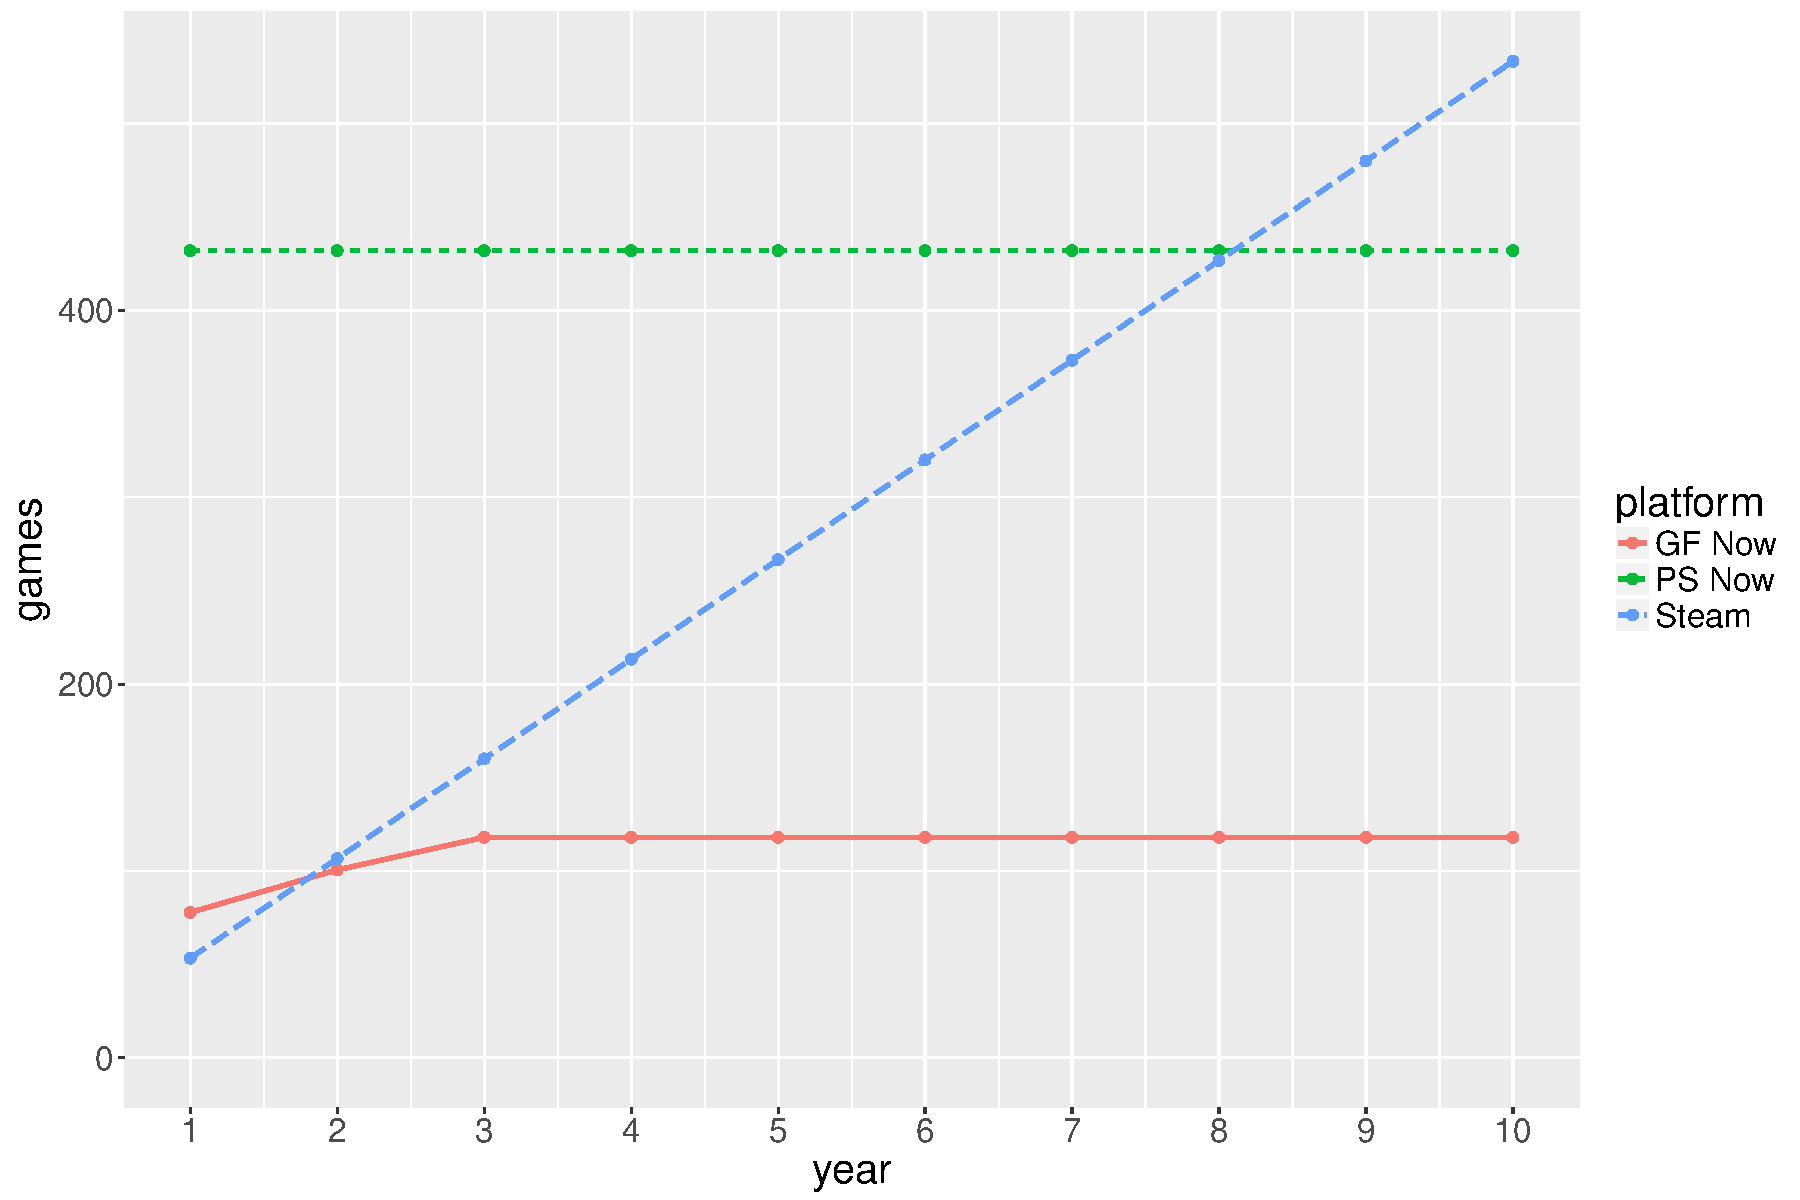
\includegraphics[width=1.0\columnwidth]{images/games-over-year.pdf}
	\caption{Number of affordable games per platform, assuming a yearly customer expenditure of \SI{500}{\EUR}.}
\label{fig:games-over-years}
\end{figure}

Fig.~\ref{fig:games-over-years} depicts this example over ten years. The continual subscription costs limit the remaining budget for additional rental titles until the maximum number of titles is reached with that particular service, whereas the number of titles from \steam will just climb steadily. The benefits of a multi-year commitment to these Cloud Gaming services therefore seem to be very limited, especially when considering, that no games are retained after ending the subscription.


%%%%%%%%%%%%%%%%%%%%%%%%%%%%%%%%%%%%%%%%%%%%%%%%%%%%%%%%%%%%%%%%%%%%%%%%%%%%%%%%
\subsection{Discussion}

Summing this section up, the investigated simple engagement metrics somewhat expose the difference between an open market platform and the curated-by-necessity cloud gaming services. The size and sales-based price model of \steam poses challenges for direct competitors such as \gfnow. Services that cater to different audiences, such as \psnow which positions itself as a backwards compatibility service, may have more success in this regard. However, the limited target audience of \psnow becomes even narrower when the high subscription costs are taken into account, diminishing the benefits for many, not even considering the additional quality challenges that streaming video games brings along. All in all this may make curated Cloud Gaming services financially unattractive for the service's operator as is discussed in the following section.

% \todo[inline]{PZ: Ist Grafik \ref{fig:games-over-years} die Basis fuer die Steigung bei ps now usw. ab dem Eintritt in Fig.~\ref{fig:gamesperyear-over-budget}. Ps now wuerde ich als Club Good sehen.}
% \todo[inline]{FM: psnow/clubgood in the sense of a backwards compatibility service for devices that do not have native access to the streamed titles?.}

%PS Now specifically caters towards older titles and backwards compatibility, may find a niche here
% wer ist die zielgruppe?
% was ist die beste platform?
% gibt es eine mainstream platform?
% unterschiedliche ausrichtungen?





% metacritic titles:
% PC 16192
% PS4 817
% XB1 588
% WiiU 474
% 3DS 871
% GFNOW 68
% PSNOW 243
% STEAM 7749



% \begin{figure}[!t]
% 	\centering
% 	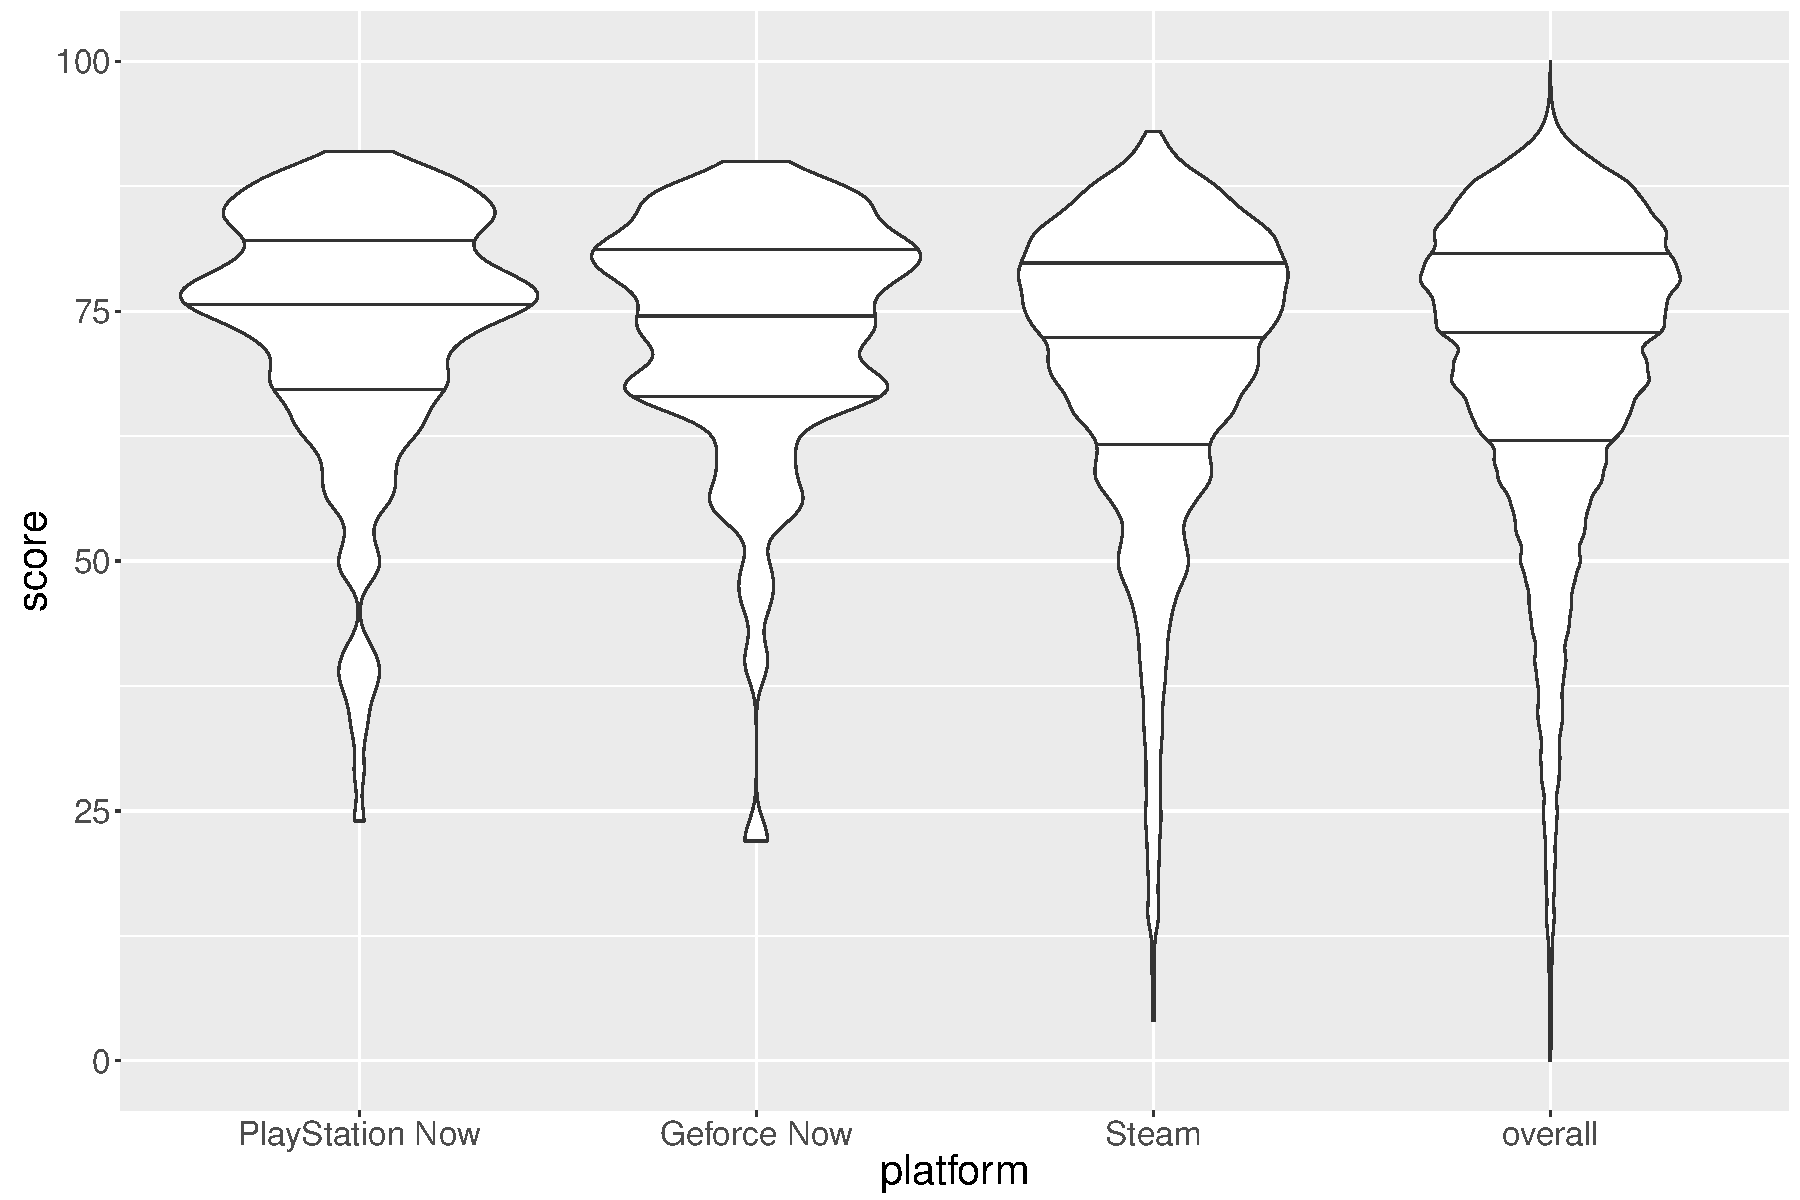
\includegraphics[width=1.0\columnwidth]{images/scores-by-platform-violin-userscore.pdf}
% 	\caption{Distribution of Metacritic user scores across the investigated platforms, depicted as violin plot with $25\%$, $50\%$, $75\%$ quantiles drawn.}
% \label{fig:userscores-by-platform}
% \end{figure}


% \subsection{E2E Lag}
% End-to-End Lag Model and Simulation in R. Now a standalone (submitted) paper at \url{https://github.com/mas-ude/onlinegame-lag-sim}. Can be referenced to argue the need for low E2E lag (meaning low network delay, but also the need for high fps).


%\item Graphical fidelity
%\item , tightness/precision/quality of controls and game mechanics, e2e lag
%\item Story?
%\item Other popularity measures? %(e.g. steamspy owner data?)
%\item Hardware requirements of games?
%\item Game costs and price history



% Caution: 
% Steam means game ownership
% PS/GF Now means only games during subscription plus permanent rental as long the sub is active(?)
% Additionally, PS Now means renting for 30 days